\section{Analysis}
\label{sec:analysis}

The preceding sections establish that \method achieves high simulation fidelity (Table~\ref{tab:main_results}) and enables effective downstream agent training (\S\ref{sec:applications}).
This section asks \emph{how} the model arrives at accurate predictions and \emph{what} changes during RL training.
We examine LWM reasoning patterns in the model's chain-of-thought (\S\ref{sec:analysis:reasoning}) and micro-level fidelity improvements driven by RL (\S\ref{sec:analysis:fidelity}).

\subsection{LWM Reasoning Patterns}
\label{sec:analysis:reasoning}


\begin{figure*}[t]
    \centering
    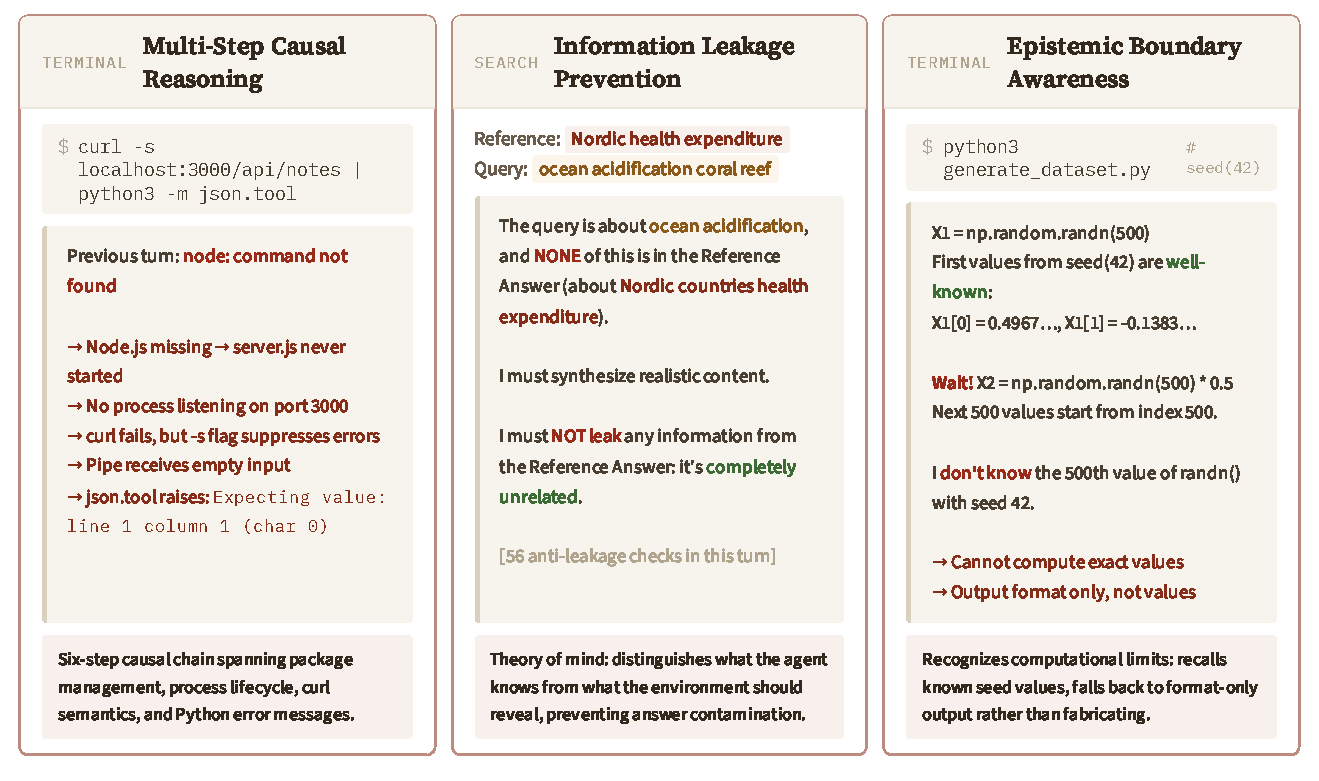
\includegraphics[width=\linewidth]{figures/lwm_reasoning_patterns.pdf}
    \caption{Representative LWM reasoning patterns from \method-397B-A17B's thinking traces.
    \textbf{Left:} Multi-step causal reasoning in Terminal, where a chain spans package management, process lifecycle, curl semantics, and Python errors.
    \textbf{Center:} Information leakage prevention in Search, where the model distinguishes what the agent knows from what the environment should reveal to prevent answer contamination.
    \textbf{Right:} Epistemic boundary awareness in Terminal, where the model recognizes computational limits and falls back to format-only output rather than fabricating unknowable values.
    }
    \label{fig:reasoning_patterns}
\end{figure*}


\method generates a chain-of-thought (thinking trace) before each predicted environment observation.
We analyze 129 thinking traces across four text-based domains from curated demonstration trajectories, covering 32 turns each in Terminal, MCP, and Search, and 33 turns in SWE.
Figure~\ref{fig:reasoning_patterns} illustrates three representative patterns and reports aggregate statistics.

\paragraph{Deliberative Self-Correction.}
The model uses ``Wait!'' as an explicit cognitive interrupt to re-examine an intermediate prediction and revise before committing.
Across 129 turns, we count 1{,}347 such interrupts (10.4 per turn on average; peak: 56 in a single SWE turn).
Terminal and MCP exhibit the highest rates (16.9 and 12.7 per turn), reflecting deeper state-tracking demands.
The self-corrections decompose into three functional subtypes:
\emph{factual} (catching an incorrect API response format),
\emph{epistemological} (recognizing the limit of in-context computation, as in the \texttt{np.random.seed(42)} example of Figure~\ref{fig:reasoning_patterns}), and
\emph{perspective-taking} (modeling the evaluator's intent or the agent's knowledge state).
This behavior converts environment prediction from single-pass generation into constrained satisfiability search.

\paragraph{Information Leakage Prevention.}
In the Search domain, the model holds a reference answer that the agent is trying to find.
When the agent's query is unrelated to this answer, the model explicitly prevents leakage: it identifies the topic mismatch and ensures that generated snippets do not accidentally reveal the target information (Figure~\ref{fig:reasoning_patterns}, center).
This is the world-model equivalent of theory of mind: the model distinguishes what the \emph{agent} knows from what the \emph{environment} should reveal.

\paragraph{Multi-Step Causal Reasoning.}
The model constructs causal chains that span multiple system abstractions.
In one Terminal example, predicting the output of \texttt{curl -s localhost:3000 | python3 -m json.tool} requires a six-step chain: Node.js missing $\to$ server never started $\to$ no listener on port 3000 $\to$ \texttt{curl} fails silently (\texttt{-s} flag) $\to$ pipe receives empty input $\to$ \texttt{json.tool} raises a specific \texttt{JSONDecodeError}.
Each step draws on different system knowledge (package management, process lifecycle, curl semantics, Python error messages), yet the model chains them correctly.
This internalized causal simulation is the mechanism through which world-model training improves downstream agent performance: an agent with this knowledge can anticipate failures before executing actions.

\subsection{RL Enhances Micro-Level Simulation Fidelity}
\label{sec:analysis:fidelity}

\begin{figure*}[t]
    \centering
    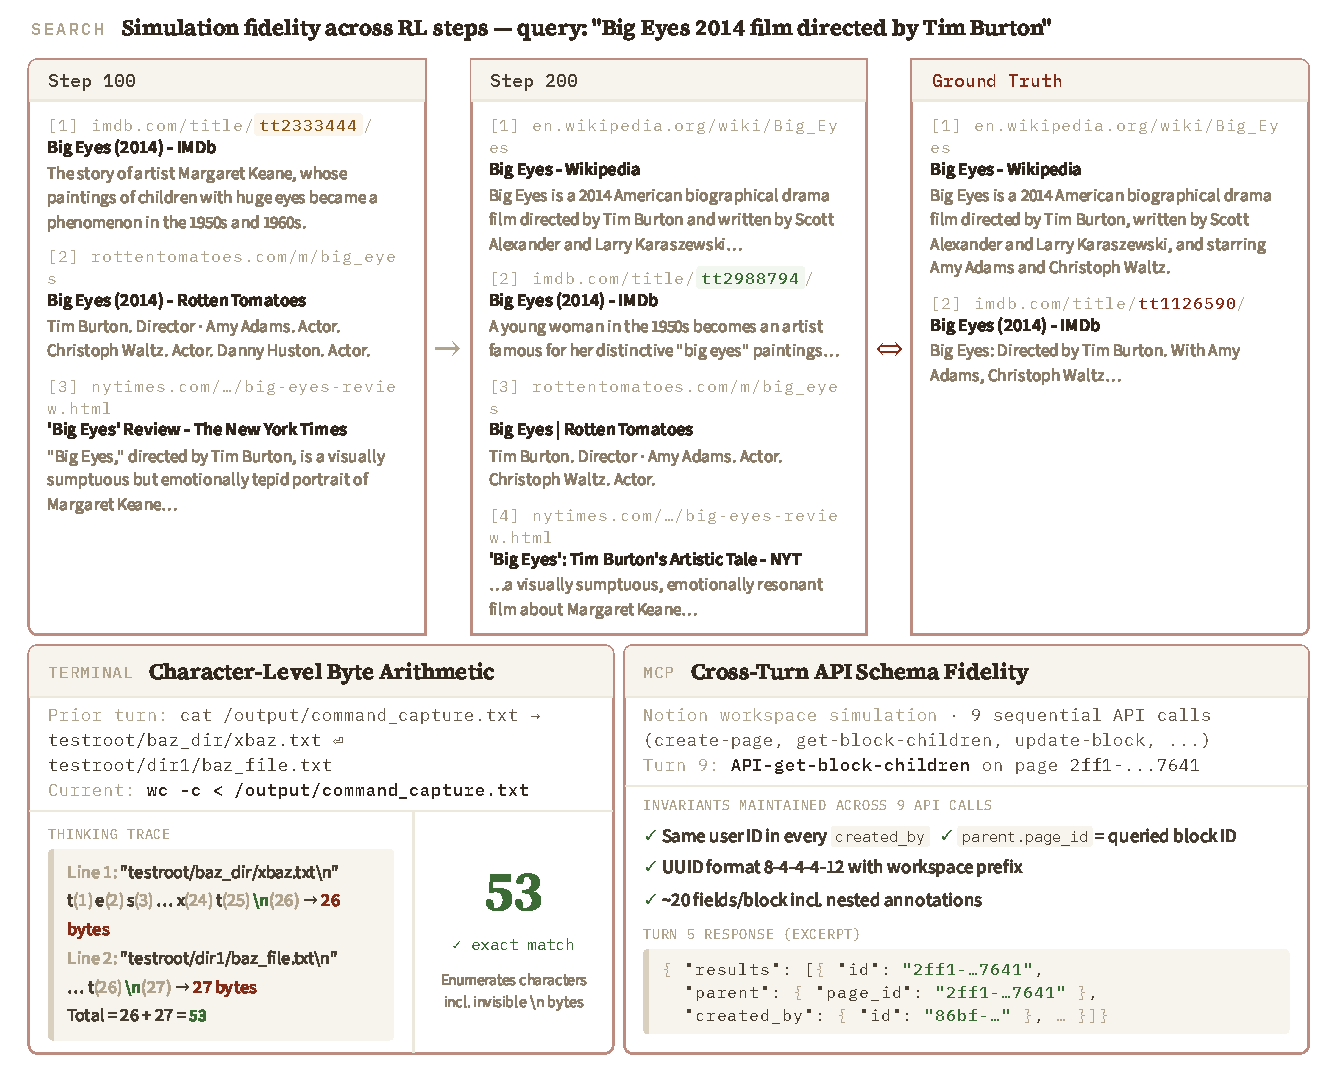
\includegraphics[width=\linewidth]{figures/rl_fidelity_progression.pdf}
    \caption{Micro-level fidelity improvements during RL training.
    \textbf{Top:} Search domain: evolution of a single sample across RL steps. URL identifiers, source diversity, and snippet specificity all improve, despite occupying a tiny fraction of total output tokens.
    \textbf{Bottom left:} Terminal domain: the model performs exact byte-level arithmetic by enumerating characters including invisible newlines.
    \textbf{Bottom right:} MCP domain: the model maintains cross-turn schema consistency (user IDs, parent-child references, UUID formats) across nine Notion API calls.
    }
    \label{fig:rl_fidelity}
\end{figure*}

Turn-level evaluation scores (\S\ref{sec:exp:main}) capture aggregate quality, but RL training also improves fidelity at a much finer granularity: individual URL identifiers, byte-level arithmetic, and cross-turn API schema consistency.
Figure~\ref{fig:rl_fidelity} illustrates these micro-level improvements.

\paragraph{Search: URL Realism across RL Steps.}
We trace a single Search-domain sample across RL checkpoints (Figure~\ref{fig:rl_fidelity}, top).
At Step~100, the model generates an IMDB URL with a plausible but synthetic title identifier (\texttt{tt2333444}) and reasonable snippets.
By Step~200, the identifier shifts to \texttt{tt2988794}, sources appear in natural ranking order (Wikipedia first, then IMDB, NYT, Rotten Tomatoes), and snippets contain query-specific factual detail that closely mirrors the ground truth.
URL identifiers are a negligible fraction of total response tokens, yet RL enhances even these low-salience details, suggesting that the reward signal propagates below the granularity of explicit reward dimensions.

\paragraph{Terminal: Character-Level Byte Arithmetic.}
In a multi-turn trajectory, the model sees file content displayed by \texttt{cat} in an earlier turn, then must predict the output of \texttt{wc -c} several turns later.
Rather than generating a plausible number, the model enumerates individual characters in its thinking trace, including invisible \texttt{\textbackslash n} bytes, and arrives at the exact count (53 bytes) through letter-by-letter arithmetic (Figure~\ref{fig:rl_fidelity}, bottom left).
In other examples, the model satisfies cryptographic invariants (identical files $\to$ identical SHA256 hashes) while simultaneously respecting Unix pipeline semantics (\texttt{tee} to a nonexistent directory fails without affecting stdout).

\paragraph{MCP: API Schema Fidelity.}
In an MCP trajectory simulating a Notion workspace (Figure~\ref{fig:rl_fidelity}, bottom right), the model maintains perfect consistency across nine sequential API calls: the same user identifier appears in every \texttt{created\_by} field, each block's \texttt{parent.page\_id} matches the queried block ID, and the full Notion schema ($\sim$20 fields per block) is reproduced without omissions.
The model implements a stateful in-context database, maintaining referential integrity across dozens of nested JSON objects.
